\documentclass[oneside]{book}

% Packages required by doxygen
\usepackage{fixltx2e}
\usepackage{calc}
\usepackage{doxygen}
\usepackage{graphicx}
\usepackage[utf8]{inputenc}
\usepackage{makeidx}
\usepackage{multicol}
\usepackage{multirow}
\PassOptionsToPackage{warn}{textcomp}
\usepackage{textcomp}
\usepackage[nointegrals]{wasysym}
\usepackage[table]{xcolor}

% Font selection
\usepackage[T1]{fontenc}
\usepackage{mathptmx}
\usepackage[scaled=.90]{helvet}
\usepackage{courier}
\usepackage{amssymb}
\usepackage{sectsty}
\renewcommand{\familydefault}{\sfdefault}
\allsectionsfont{%
  \fontseries{bc}\selectfont%
  \color{darkgray}%
}
\renewcommand{\DoxyLabelFont}{%
  \fontseries{bc}\selectfont%
  \color{darkgray}%
}
\newcommand{\+}{\discretionary{\mbox{\scriptsize$\hookleftarrow$}}{}{}}

% Page & text layout
\usepackage{geometry}
\geometry{%
  a4paper,%
  top=2.5cm,%
  bottom=2.5cm,%
  left=2.5cm,%
  right=2.5cm%
}
\tolerance=750
\hfuzz=15pt
\hbadness=750
\setlength{\emergencystretch}{15pt}
\setlength{\parindent}{0cm}
\setlength{\parskip}{0.2cm}
\makeatletter
\renewcommand{\paragraph}{%
  \@startsection{paragraph}{4}{0ex}{-1.0ex}{1.0ex}{%
    \normalfont\normalsize\bfseries\SS@parafont%
  }%
}
\renewcommand{\subparagraph}{%
  \@startsection{subparagraph}{5}{0ex}{-1.0ex}{1.0ex}{%
    \normalfont\normalsize\bfseries\SS@subparafont%
  }%
}
\makeatother

% Headers & footers
\usepackage{fancyhdr}
\pagestyle{fancyplain}
\fancyhead[LE]{\fancyplain{}{\bfseries\thepage}}
\fancyhead[CE]{\fancyplain{}{}}
\fancyhead[RE]{\fancyplain{}{\bfseries\leftmark}}
\fancyhead[LO]{\fancyplain{}{\bfseries\rightmark}}
\fancyhead[CO]{\fancyplain{}{}}
\fancyhead[RO]{\fancyplain{}{\bfseries\thepage}}
\fancyfoot[LE]{\fancyplain{}{}}
\fancyfoot[CE]{\fancyplain{}{}}
\fancyfoot[RE]{\fancyplain{}{\bfseries\scriptsize Generated on Wed Feb 24 2016 00\+:40\+:53 for Implementation of Red Black Trees in C by Doxygen }}
\fancyfoot[LO]{\fancyplain{}{\bfseries\scriptsize Generated on Wed Feb 24 2016 00\+:40\+:53 for Implementation of Red Black Trees in C by Doxygen }}
\fancyfoot[CO]{\fancyplain{}{}}
\fancyfoot[RO]{\fancyplain{}{}}
\renewcommand{\footrulewidth}{0.4pt}
\renewcommand{\chaptermark}[1]{%
  \markboth{#1}{}%
}
\renewcommand{\sectionmark}[1]{%
  \markright{\thesection\ #1}%
}

% Indices & bibliography
\usepackage{natbib}
\usepackage[titles]{tocloft}
\setcounter{tocdepth}{3}
\setcounter{secnumdepth}{5}
\makeindex

% Hyperlinks (required, but should be loaded last)
\usepackage{ifpdf}
\ifpdf
  \usepackage[pdftex,pagebackref=true]{hyperref}
\else
  \usepackage[ps2pdf,pagebackref=true]{hyperref}
\fi
\hypersetup{%
  colorlinks=true,%
  linkcolor=blue,%
  citecolor=blue,%
  unicode%
}

% Custom commands
\newcommand{\clearemptydoublepage}{%
  \newpage{\pagestyle{empty}\cleardoublepage}%
}


%===== C O N T E N T S =====

\begin{document}

% Titlepage & ToC
\hypersetup{pageanchor=false,
             bookmarks=true,
             bookmarksnumbered=true,
             pdfencoding=unicode
            }
\pagenumbering{roman}
\begin{titlepage}
\vspace*{7cm}
\begin{center}%
{\Large Implementation of Red Black Trees in C \\[1ex]\large Anant Maheshwari 13\+C\+O111 Shrukul Habib 13\+C\+O143 }\\
\vspace*{1cm}
{\large Generated by Doxygen 1.8.7}\\
\vspace*{0.5cm}
{\small Wed Feb 24 2016 00:40:53}\\
\end{center}
\end{titlepage}
\clearemptydoublepage
\tableofcontents
\clearemptydoublepage
\pagenumbering{arabic}
\hypersetup{pageanchor=true}

%--- Begin generated contents ---
\chapter{Class Index}
\section{Class List}
Here are the classes, structs, unions and interfaces with brief descriptions\+:\begin{DoxyCompactList}
\item\contentsline{section}{\hyperlink{classBinomialHeap}{Binomial\+Heap} \\*Binomial Heap Data Structure class }{\pageref{classBinomialHeap}}{}
\item\contentsline{section}{\hyperlink{classFibonacciHeap}{Fibonacci\+Heap} \\*Fibonacci Heap Data Structure class }{\pageref{classFibonacciHeap}}{}
\item\contentsline{section}{\hyperlink{structnode}{node} \\*$\ast$-\/-\/-\/-\/-\/-\/-\/-\/-\/-\/-\/-\/-\/-\/-\/-\/-\/-\/-\/-\/-\/-\/-\/-\/-\/------B\+I\+N\+O\+M\+I\+AL H\+E\+A\+P-\/-\/-\/-\/-\/-\/-\/-\/-\/-\/-\/-\/-\/-\/-\/-\/-\/-\/-\/-\/-\/-\/-\/-\/-\/-\/-\/-\/-\/-\/-\/-\/-\/-\/-\/-\/-\/-\/-\/-\/-\/-\/-\/-\/-\/-\/-\/-\/-\/-\/------$\ast$/ }{\pageref{structnode}}{}
\item\contentsline{section}{\hyperlink{structnodef}{nodef} \\*$\ast$-\/-\/-\/-\/-\/-\/-\/-\/-\/-\/-\/-\/-\/-\/-\/-\/-\/-\/-\/-\/-\/-\/-\/-\/-\/-\/------F\+I\+B\+O\+N\+A\+C\+CI H\+E\+A\+P-\/-\/-\/-\/-\/-\/-\/-\/-\/-\/-\/-\/-\/-\/-\/-\/-\/-\/-\/-\/-\/-\/-\/-\/-\/-\/-\/-\/-\/-\/-\/-\/-\/-\/-\/-\/-\/-\/-\/-\/-\/-\/-\/-\/-\/-\/-\/-\/-\/-\/-\/-\/-\/-\/-\/-\/-\/-\/-\/-\/-\/-\/-\/------$\ast$/ }{\pageref{structnodef}}{}
\end{DoxyCompactList}

\chapter{File Index}
\section{File List}
Here is a list of all documented files with brief descriptions\+:\begin{DoxyCompactList}
\item\contentsline{section}{\hyperlink{red__black__tree_8c}{red\+\_\+black\+\_\+tree.\+c} \\*Implementation of Red Black Tree }{\pageref{red__black__tree_8c}}{}
\end{DoxyCompactList}

\chapter{Class Documentation}
\hypertarget{structnode}{\section{node Struct Reference}
\label{structnode}\index{node@{node}}
}


Collaboration diagram for node\+:\nopagebreak
\begin{figure}[H]
\begin{center}
\leavevmode
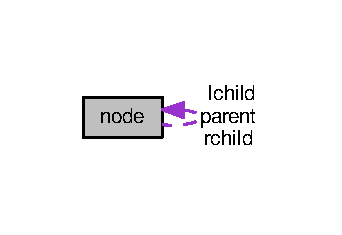
\includegraphics[width=164pt]{structnode__coll__graph}
\end{center}
\end{figure}
\subsection*{Public Types}
\begin{DoxyCompactItemize}
\item 
\hypertarget{structnode_affe9650e53b0efaa6d69372b45d795bd}{enum \{ {\bfseries black}, 
{\bfseries red}
 \}}\label{structnode_affe9650e53b0efaa6d69372b45d795bd}

\end{DoxyCompactItemize}
\subsection*{Public Attributes}
\begin{DoxyCompactItemize}
\item 
\hypertarget{structnode_a883641a3dd856c38125e6a08db4e66af}{enum node\+:: \{ ... \}  {\bfseries colour}}\label{structnode_a883641a3dd856c38125e6a08db4e66af}

\item 
int \hyperlink{structnode_ac8973feda870a119ccdc25910254db0c}{info}
\item 
struct \hyperlink{structnode}{node} $\ast$ \hyperlink{structnode_a5e9a6db5c18bb131ca4b72a1ff575ad8}{lchild}
\item 
struct \hyperlink{structnode}{node} $\ast$ \hyperlink{structnode_aa1ed9628cfc90de6f68ff88ddf9350fa}{rchild}
\item 
struct \hyperlink{structnode}{node} $\ast$ \hyperlink{structnode_a05e4fe9e0177ba2d8dbd2c487cfddd53}{parent}
\end{DoxyCompactItemize}


\subsection{Member Data Documentation}
\hypertarget{structnode_ac8973feda870a119ccdc25910254db0c}{\index{node@{node}!info@{info}}
\index{info@{info}!node@{node}}
\subsubsection[{info}]{\setlength{\rightskip}{0pt plus 5cm}int node\+::info}}\label{structnode_ac8973feda870a119ccdc25910254db0c}
Stores whether the node is red or black \hypertarget{structnode_a5e9a6db5c18bb131ca4b72a1ff575ad8}{\index{node@{node}!lchild@{lchild}}
\index{lchild@{lchild}!node@{node}}
\subsubsection[{lchild}]{\setlength{\rightskip}{0pt plus 5cm}struct {\bf node}$\ast$ node\+::lchild}}\label{structnode_a5e9a6db5c18bb131ca4b72a1ff575ad8}
Stores the value of the node \hypertarget{structnode_a05e4fe9e0177ba2d8dbd2c487cfddd53}{\index{node@{node}!parent@{parent}}
\index{parent@{parent}!node@{node}}
\subsubsection[{parent}]{\setlength{\rightskip}{0pt plus 5cm}struct {\bf node}$\ast$ node\+::parent}}\label{structnode_a05e4fe9e0177ba2d8dbd2c487cfddd53}
Pointer of the right node \hypertarget{structnode_aa1ed9628cfc90de6f68ff88ddf9350fa}{\index{node@{node}!rchild@{rchild}}
\index{rchild@{rchild}!node@{node}}
\subsubsection[{rchild}]{\setlength{\rightskip}{0pt plus 5cm}struct {\bf node}$\ast$ node\+::rchild}}\label{structnode_aa1ed9628cfc90de6f68ff88ddf9350fa}
Pointer of the left node 

The documentation for this struct was generated from the following file\+:\begin{DoxyCompactItemize}
\item 
\hyperlink{red__black__tree_8c}{red\+\_\+black\+\_\+tree.\+c}\end{DoxyCompactItemize}

\chapter{File Documentation}
\hypertarget{red__black__tree_8c}{\section{red\+\_\+black\+\_\+tree.\+c File Reference}
\label{red__black__tree_8c}\index{red\+\_\+black\+\_\+tree.\+c@{red\+\_\+black\+\_\+tree.\+c}}
}


Implementation of Red Black Tree.  


{\ttfamily \#include $<$stdio.\+h$>$}\\*
{\ttfamily \#include $<$stdlib.\+h$>$}\\*
Include dependency graph for red\+\_\+black\+\_\+tree.\+c\+:\nopagebreak
\begin{figure}[H]
\begin{center}
\leavevmode
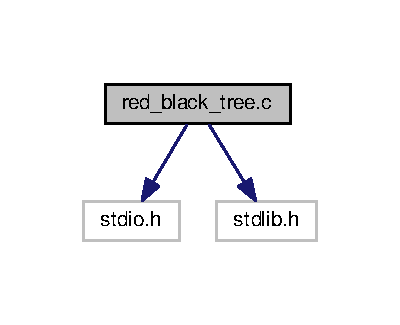
\includegraphics[width=192pt]{red__black__tree_8c__incl}
\end{center}
\end{figure}
\subsection*{Classes}
\begin{DoxyCompactItemize}
\item 
struct \hyperlink{structnode}{node}
\end{DoxyCompactItemize}
\subsection*{Functions}
\begin{DoxyCompactItemize}
\item 
int \hyperlink{red__black__tree_8c_a2624fa1cdd67434b8466330d6da136cb}{find} (int item, struct \hyperlink{structnode}{node} $\ast$$\ast$loc)
\begin{DoxyCompactList}\small\item\em Check whether a node with the given value exists in the tree or not. \end{DoxyCompactList}\item 
void \hyperlink{red__black__tree_8c_af0d230db694cce552cc1f2d9ace36790}{insert} (int item)
\begin{DoxyCompactList}\small\item\em Inserts a new node. Incase of duplicate node, error is displayed. \end{DoxyCompactList}\item 
void \hyperlink{red__black__tree_8c_a4117a1fa4bbc89c43cde2db723675185}{insert\+\_\+balance} (struct \hyperlink{structnode}{node} $\ast$nptr)
\begin{DoxyCompactList}\small\item\em The function performs series of rotations needed after node insertion. \end{DoxyCompactList}\item 
void \hyperlink{red__black__tree_8c_a9929d6460fc3777d7ed5370228821f00}{del} (int item)
\begin{DoxyCompactList}\small\item\em Delete a node from the tree. \end{DoxyCompactList}\item 
void \hyperlink{red__black__tree_8c_a60538a082c5e9d7ee8bf3a8875a9a046}{del\+\_\+balance} (struct \hyperlink{structnode}{node} $\ast$ptr)
\begin{DoxyCompactList}\small\item\em The function performs series of rotations needed after node deletion. \end{DoxyCompactList}\item 
void \hyperlink{red__black__tree_8c_a4dc9f3f6d87d9c09d27a08d57467fd37}{rotate\+\_\+left} (struct \hyperlink{structnode}{node} $\ast$ptr)
\begin{DoxyCompactList}\small\item\em Rotates the tree about the given node in left direction. \end{DoxyCompactList}\item 
void \hyperlink{red__black__tree_8c_a0adc3d0efa320d6e4f2d833f61e9b105}{rotate\+\_\+right} (struct \hyperlink{structnode}{node} $\ast$ptr)
\begin{DoxyCompactList}\small\item\em Rotates the tree about the given node in right direction. \end{DoxyCompactList}\item 
struct \hyperlink{structnode}{node} $\ast$ \hyperlink{red__black__tree_8c_a832bde6c280220c1d6ab2bb7dc3b9c37}{succ} (struct \hyperlink{structnode}{node} $\ast$ptr)
\begin{DoxyCompactList}\small\item\em Finds the inorder successor of the given node. \end{DoxyCompactList}\item 
void \hyperlink{red__black__tree_8c_af196af0377ad9c6c183cecbea834b5fd}{inorder} (struct \hyperlink{structnode}{node} $\ast$ptr)
\begin{DoxyCompactList}\small\item\em Displays Inorder traversal of the tree. \end{DoxyCompactList}\item 
void \hyperlink{red__black__tree_8c_a7b2e47b8cf80a34f26da732cba791a85}{display} (struct \hyperlink{structnode}{node} $\ast$ptr, int level)
\begin{DoxyCompactList}\small\item\em Level order traversal of the tree. \end{DoxyCompactList}\item 
int \hyperlink{red__black__tree_8c_ae66f6b31b5ad750f1fe042a706a4e3d4}{main} ()
\begin{DoxyCompactList}\small\item\em The Main Function of the Program. \end{DoxyCompactList}\end{DoxyCompactItemize}
\subsection*{Variables}
\begin{DoxyCompactItemize}
\item 
\hypertarget{red__black__tree_8c_a4c4817f1c5c2801859d1ded04bf23dce}{struct \hyperlink{structnode}{node} $\ast$ {\bfseries root}}\label{red__black__tree_8c_a4c4817f1c5c2801859d1ded04bf23dce}

\item 
struct \hyperlink{structnode}{node} $\ast$ \hyperlink{red__black__tree_8c_a540cb45ebb5713fdbd4ead62f41d35d6}{sentinel}
\end{DoxyCompactItemize}


\subsection{Detailed Description}
Implementation of Red Black Tree. 

\begin{DoxyAuthor}{Author}
Shrukul Habib 13\+C\+O143 

Anant Maheshwari 13\+C\+O111 
\end{DoxyAuthor}


\subsection{Function Documentation}
\hypertarget{red__black__tree_8c_a9929d6460fc3777d7ed5370228821f00}{\index{red\+\_\+black\+\_\+tree.\+c@{red\+\_\+black\+\_\+tree.\+c}!del@{del}}
\index{del@{del}!red\+\_\+black\+\_\+tree.\+c@{red\+\_\+black\+\_\+tree.\+c}}
\subsubsection[{del}]{\setlength{\rightskip}{0pt plus 5cm}void del (
\begin{DoxyParamCaption}
\item[{int}]{item}
\end{DoxyParamCaption}
)}}\label{red__black__tree_8c_a9929d6460fc3777d7ed5370228821f00}


Delete a node from the tree. 


\begin{DoxyParams}{Parameters}
{\em item} & Value of the node to be deleted\\
\hline
\end{DoxyParams}
\begin{DoxyReturn}{Returns}
Doesn't return anything, void. 
\end{DoxyReturn}
\hypertarget{red__black__tree_8c_a60538a082c5e9d7ee8bf3a8875a9a046}{\index{red\+\_\+black\+\_\+tree.\+c@{red\+\_\+black\+\_\+tree.\+c}!del\+\_\+balance@{del\+\_\+balance}}
\index{del\+\_\+balance@{del\+\_\+balance}!red\+\_\+black\+\_\+tree.\+c@{red\+\_\+black\+\_\+tree.\+c}}
\subsubsection[{del\+\_\+balance}]{\setlength{\rightskip}{0pt plus 5cm}void del\+\_\+balance (
\begin{DoxyParamCaption}
\item[{struct {\bf node} $\ast$}]{ptr}
\end{DoxyParamCaption}
)}}\label{red__black__tree_8c_a60538a082c5e9d7ee8bf3a8875a9a046}


The function performs series of rotations needed after node deletion. 


\begin{DoxyParams}{Parameters}
{\em ptr} & value of the node to be deleted\\
\hline
\end{DoxyParams}
\begin{DoxyReturn}{Returns}
Doesn't return anything, void. 
\end{DoxyReturn}
\hypertarget{red__black__tree_8c_a7b2e47b8cf80a34f26da732cba791a85}{\index{red\+\_\+black\+\_\+tree.\+c@{red\+\_\+black\+\_\+tree.\+c}!display@{display}}
\index{display@{display}!red\+\_\+black\+\_\+tree.\+c@{red\+\_\+black\+\_\+tree.\+c}}
\subsubsection[{display}]{\setlength{\rightskip}{0pt plus 5cm}void display (
\begin{DoxyParamCaption}
\item[{struct {\bf node} $\ast$}]{ptr, }
\item[{int}]{level}
\end{DoxyParamCaption}
)}}\label{red__black__tree_8c_a7b2e47b8cf80a34f26da732cba791a85}


Level order traversal of the tree. 


\begin{DoxyParams}{Parameters}
{\em ptr} & The pointer of the root node \\
\hline
{\em level} & The Level of the the current node (1, if starting from root)\\
\hline
\end{DoxyParams}
\begin{DoxyReturn}{Returns}
Doesn't return anything, void. 
\end{DoxyReturn}
\hypertarget{red__black__tree_8c_a2624fa1cdd67434b8466330d6da136cb}{\index{red\+\_\+black\+\_\+tree.\+c@{red\+\_\+black\+\_\+tree.\+c}!find@{find}}
\index{find@{find}!red\+\_\+black\+\_\+tree.\+c@{red\+\_\+black\+\_\+tree.\+c}}
\subsubsection[{find}]{\setlength{\rightskip}{0pt plus 5cm}int find (
\begin{DoxyParamCaption}
\item[{int}]{item, }
\item[{struct {\bf node} $\ast$$\ast$}]{loc}
\end{DoxyParamCaption}
)}}\label{red__black__tree_8c_a2624fa1cdd67434b8466330d6da136cb}


Check whether a node with the given value exists in the tree or not. 


\begin{DoxyParams}{Parameters}
{\em item} & The value of the node to be checked \\
\hline
{\em loc} & The location of the found node \\
\hline
\end{DoxyParams}
\begin{DoxyReturn}{Returns}
Doesn't return anything, void. 
\end{DoxyReturn}
\hypertarget{red__black__tree_8c_af196af0377ad9c6c183cecbea834b5fd}{\index{red\+\_\+black\+\_\+tree.\+c@{red\+\_\+black\+\_\+tree.\+c}!inorder@{inorder}}
\index{inorder@{inorder}!red\+\_\+black\+\_\+tree.\+c@{red\+\_\+black\+\_\+tree.\+c}}
\subsubsection[{inorder}]{\setlength{\rightskip}{0pt plus 5cm}void inorder (
\begin{DoxyParamCaption}
\item[{struct {\bf node} $\ast$}]{ptr}
\end{DoxyParamCaption}
)}}\label{red__black__tree_8c_af196af0377ad9c6c183cecbea834b5fd}


Displays Inorder traversal of the tree. 


\begin{DoxyParams}{Parameters}
{\em ptr} & The pointer of the root node.\\
\hline
\end{DoxyParams}
\begin{DoxyReturn}{Returns}
Doesn't return anything, void. 
\end{DoxyReturn}
\hypertarget{red__black__tree_8c_af0d230db694cce552cc1f2d9ace36790}{\index{red\+\_\+black\+\_\+tree.\+c@{red\+\_\+black\+\_\+tree.\+c}!insert@{insert}}
\index{insert@{insert}!red\+\_\+black\+\_\+tree.\+c@{red\+\_\+black\+\_\+tree.\+c}}
\subsubsection[{insert}]{\setlength{\rightskip}{0pt plus 5cm}void insert (
\begin{DoxyParamCaption}
\item[{int}]{item}
\end{DoxyParamCaption}
)}}\label{red__black__tree_8c_af0d230db694cce552cc1f2d9ace36790}


Inserts a new node. Incase of duplicate node, error is displayed. 


\begin{DoxyParams}{Parameters}
{\em item} & The value of the node to be inserted.\\
\hline
\end{DoxyParams}
\begin{DoxyReturn}{Returns}
Doesn't return anything, void. 
\end{DoxyReturn}
\hypertarget{red__black__tree_8c_a4117a1fa4bbc89c43cde2db723675185}{\index{red\+\_\+black\+\_\+tree.\+c@{red\+\_\+black\+\_\+tree.\+c}!insert\+\_\+balance@{insert\+\_\+balance}}
\index{insert\+\_\+balance@{insert\+\_\+balance}!red\+\_\+black\+\_\+tree.\+c@{red\+\_\+black\+\_\+tree.\+c}}
\subsubsection[{insert\+\_\+balance}]{\setlength{\rightskip}{0pt plus 5cm}void insert\+\_\+balance (
\begin{DoxyParamCaption}
\item[{struct {\bf node} $\ast$}]{nptr}
\end{DoxyParamCaption}
)}}\label{red__black__tree_8c_a4117a1fa4bbc89c43cde2db723675185}


The function performs series of rotations needed after node insertion. 


\begin{DoxyParams}{Parameters}
{\em nptr} & The pointer of the new node.\\
\hline
\end{DoxyParams}
\begin{DoxyReturn}{Returns}
Doesn't return anything, void. 
\end{DoxyReturn}
\hypertarget{red__black__tree_8c_ae66f6b31b5ad750f1fe042a706a4e3d4}{\index{red\+\_\+black\+\_\+tree.\+c@{red\+\_\+black\+\_\+tree.\+c}!main@{main}}
\index{main@{main}!red\+\_\+black\+\_\+tree.\+c@{red\+\_\+black\+\_\+tree.\+c}}
\subsubsection[{main}]{\setlength{\rightskip}{0pt plus 5cm}int main (
\begin{DoxyParamCaption}
{}
\end{DoxyParamCaption}
)}}\label{red__black__tree_8c_ae66f6b31b5ad750f1fe042a706a4e3d4}


The Main Function of the Program. 

for parent of root node and N\+U\+L\+L nodes \begin{DoxyReturn}{Returns}
Doesn't return anything, void. 
\end{DoxyReturn}
\hypertarget{red__black__tree_8c_a4dc9f3f6d87d9c09d27a08d57467fd37}{\index{red\+\_\+black\+\_\+tree.\+c@{red\+\_\+black\+\_\+tree.\+c}!rotate\+\_\+left@{rotate\+\_\+left}}
\index{rotate\+\_\+left@{rotate\+\_\+left}!red\+\_\+black\+\_\+tree.\+c@{red\+\_\+black\+\_\+tree.\+c}}
\subsubsection[{rotate\+\_\+left}]{\setlength{\rightskip}{0pt plus 5cm}void rotate\+\_\+left (
\begin{DoxyParamCaption}
\item[{struct {\bf node} $\ast$}]{ptr}
\end{DoxyParamCaption}
)}}\label{red__black__tree_8c_a4dc9f3f6d87d9c09d27a08d57467fd37}


Rotates the tree about the given node in left direction. 


\begin{DoxyParams}{Parameters}
{\em ptr} & The pointer of the node about which the tree is to be rotated.\\
\hline
\end{DoxyParams}
\begin{DoxyReturn}{Returns}
Doesn't return anything, void. 
\end{DoxyReturn}
\hypertarget{red__black__tree_8c_a0adc3d0efa320d6e4f2d833f61e9b105}{\index{red\+\_\+black\+\_\+tree.\+c@{red\+\_\+black\+\_\+tree.\+c}!rotate\+\_\+right@{rotate\+\_\+right}}
\index{rotate\+\_\+right@{rotate\+\_\+right}!red\+\_\+black\+\_\+tree.\+c@{red\+\_\+black\+\_\+tree.\+c}}
\subsubsection[{rotate\+\_\+right}]{\setlength{\rightskip}{0pt plus 5cm}void rotate\+\_\+right (
\begin{DoxyParamCaption}
\item[{struct {\bf node} $\ast$}]{ptr}
\end{DoxyParamCaption}
)}}\label{red__black__tree_8c_a0adc3d0efa320d6e4f2d833f61e9b105}


Rotates the tree about the given node in right direction. 


\begin{DoxyParams}{Parameters}
{\em ptr} & The pointer of the node about which the tree is to be rotated.\\
\hline
\end{DoxyParams}
\begin{DoxyReturn}{Returns}
Doesn't return anything, void. 
\end{DoxyReturn}
\hypertarget{red__black__tree_8c_a832bde6c280220c1d6ab2bb7dc3b9c37}{\index{red\+\_\+black\+\_\+tree.\+c@{red\+\_\+black\+\_\+tree.\+c}!succ@{succ}}
\index{succ@{succ}!red\+\_\+black\+\_\+tree.\+c@{red\+\_\+black\+\_\+tree.\+c}}
\subsubsection[{succ}]{\setlength{\rightskip}{0pt plus 5cm}struct {\bf node} $\ast$ succ (
\begin{DoxyParamCaption}
\item[{struct {\bf node} $\ast$}]{ptr}
\end{DoxyParamCaption}
)}}\label{red__black__tree_8c_a832bde6c280220c1d6ab2bb7dc3b9c37}


Finds the inorder successor of the given node. 


\begin{DoxyParams}{Parameters}
{\em ptr} & The pointer of the given node.\\
\hline
\end{DoxyParams}
\begin{DoxyReturn}{Returns}
The pointer of the successor node. 
\end{DoxyReturn}


\subsection{Variable Documentation}
\hypertarget{red__black__tree_8c_a540cb45ebb5713fdbd4ead62f41d35d6}{\index{red\+\_\+black\+\_\+tree.\+c@{red\+\_\+black\+\_\+tree.\+c}!sentinel@{sentinel}}
\index{sentinel@{sentinel}!red\+\_\+black\+\_\+tree.\+c@{red\+\_\+black\+\_\+tree.\+c}}
\subsubsection[{sentinel}]{\setlength{\rightskip}{0pt plus 5cm}struct {\bf node}$\ast$ sentinel}}\label{red__black__tree_8c_a540cb45ebb5713fdbd4ead62f41d35d6}
This is the pointer of the root node 
%--- End generated contents ---

% Index
\newpage
\phantomsection
\addcontentsline{toc}{chapter}{Index}
\printindex

\end{document}
